%TCIDATA{LaTeXparent=0,0,relatorio.tex}
 


\chapter{Introdução}

\label{CapIntro}

% Resumo opcional. Comentar se não usar.
\resumodocapitulo{ ``Opcional, geralmente se colocam pequenos resumos
ou citações interessantes.'' -- Murilo M. Marinho}

Esse capítulo faz uma introdução do leitor ao contexto do trabalho,
define a problemática a ser trabalhada no projeto e resume os resultados
e o manuscrito.


\section{Contextualização}

O câncer é uma doença devastadora e um problema de saúde pública que
afeta milhares de pessoas em todos os países do mundo no contexto
atual de globalização. No mundo, o câncer é responsável por mais de
seis milhões de óbitos a cada ano. 

No Brasil, a situação não é diferente. Entre 1980 e 2004, a mortalidade
causada por alguns tipos de câncer, como o de próstata, aumentou substancialmente
\cite{LuizAugustoMarcondesFonseca2010,MaximilianoRibeiroGuerra2005}.
Ainda que o câncer não seja transmissível, a recorrência dessa doença
na população brasileira é alarmante, como pode ser visto na Figura
\ref{fig:IntroducaoDistribuicaoProstata}.%
\footnote{A População Padrão Mundial é utilizada para eliminar o efeito de diferenças
etárias na população e assim possibilitar comparações de risco de
mortalidade de acordo com a faixa etária, independentemente de questões
econômicas, geográficas e temporais. Ela funciona como um grupo comum
de pesos para o cálculo de taxas padronizadas ou ajustadas \cite{1999-2003}.%
} 

\begin{figure}[h]
\hfill{}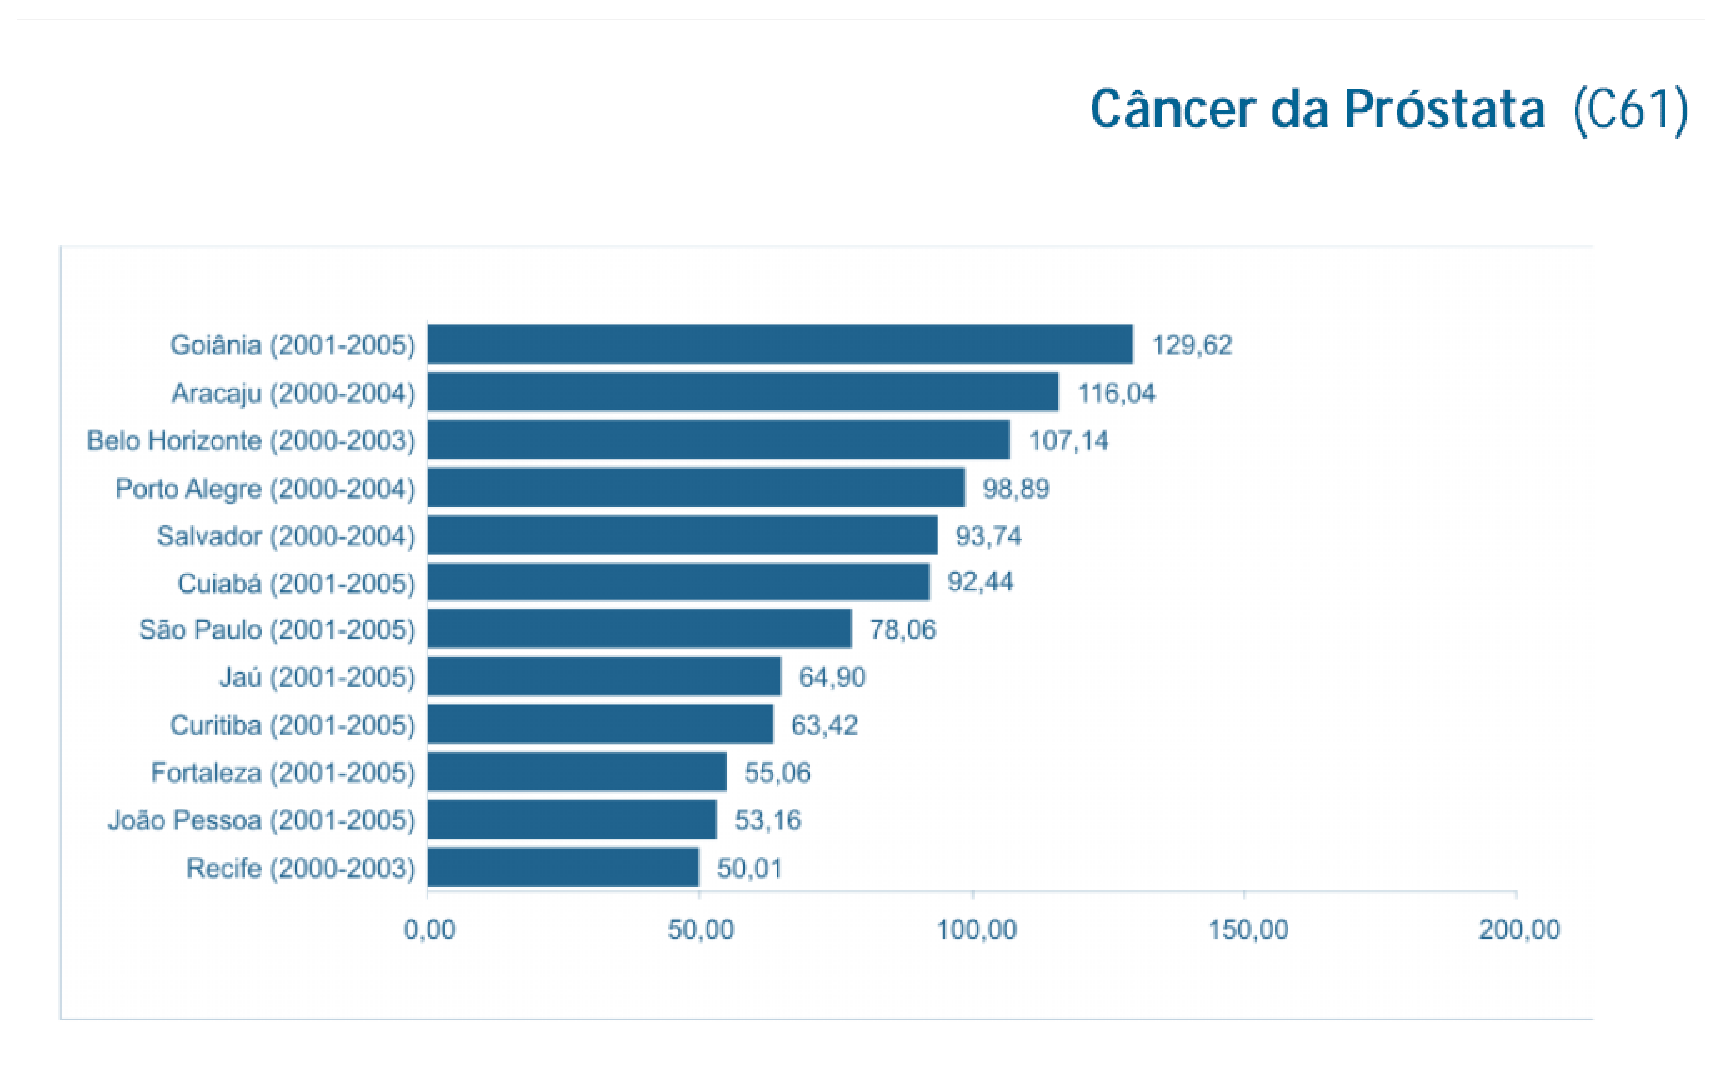
\includegraphics[scale=0.5]{figs/introducao/cancer_prostata}\hfill{}

\caption{\label{fig:IntroducaoDistribuicaoProstata}Distribuição de câncer
da próstata em diferentes cidades brasileiras. As taxas são dadas
em grupos de 100mil/ População Padrão Mundial. Fonte: \cite{INCA2005}.}
\end{figure}





\section{Definição do problema}

O problema que o trabalho pretende solucionar.


\section{Objetivos do projeto}

Quais os principais objetivos do projeto.


\section{Resultados obtidos}

Os principais resultados obtidos.


\section{Apresentação do manuscrito}

Breve resumo do manuscrito, sobre o quê cada capítulo falará posteriormente.
